\documentclass[tikz,border=2pt]{standalone}
\usepackage{amsmath}
\usepackage{amssymb}
\usepackage{pgfplots}
\pgfplotsset{compat=1.18}
\usetikzlibrary{arrows.meta}
\begin{document}
% MVA for the five-station cycle with E[S]=(2,3/2,1,3/4,1/2), V_i=1: mean populations E[L_i(n)]
% for n=0,...,12. Station 1 (bottleneck) keeps growing, the four faster stations level off.
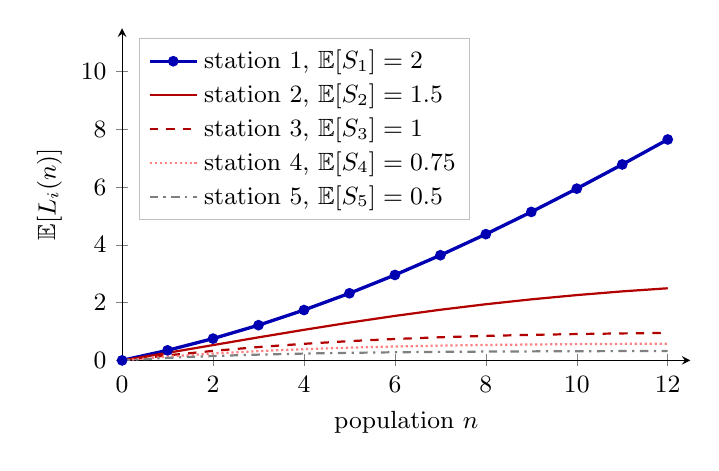
\begin{tikzpicture}[font=\small, >={Latex[length=2mm]}]
\begin{axis}[width=8.8cm, height=5.8cm, axis lines=left,
  xmin=0, xmax=12.5, ymin=0, ymax=11.5,
  xtick={0,2,4,6,8,10,12}, ytick={0,2,4,6,8,10},
  xlabel={population $n$}, ylabel={$\mathbb{E}[L_i(n)]$},
  legend pos=north west, legend cell align=left,
  legend style={draw=gray!50, font=\small}]
  \addplot[very thick, blue!70!black, mark=*, mark size=1.3pt] coordinates {(0,0.000) (1,0.348) (2,0.754) (3,1.219) (4,1.743) (5,2.323) (6,2.957) (7,3.641) (8,4.370) (9,5.140) (10,5.946) (11,6.783) (12,7.648)};
  \addlegendentry{station 1, $\mathbb{E}[S_1]=2$}
  \addplot[thick, red!70!black] coordinates {(0,0.000) (1,0.261) (2,0.529) (3,0.797) (4,1.058) (5,1.308) (6,1.540) (7,1.753) (8,1.944) (9,2.113) (10,2.261) (11,2.389) (12,2.497)};
  \addlegendentry{station 2, $\mathbb{E}[S_2]=1.5$}
  \addplot[thick, red!70!black, dashed] coordinates {(0,0.000) (1,0.174) (2,0.328) (3,0.462) (4,0.574) (5,0.667) (6,0.741) (7,0.801) (8,0.848) (9,0.884) (10,0.912) (11,0.934) (12,0.950)};
  \addlegendentry{station 3, $\mathbb{E}[S_3]=1$}
  \addplot[thick, red!50, densely dotted] coordinates {(0,0.000) (1,0.130) (2,0.237) (3,0.322) (4,0.389) (5,0.441) (6,0.481) (7,0.511) (8,0.534) (9,0.550) (10,0.563) (11,0.572) (12,0.579)};
  \addlegendentry{station 4, $\mathbb{E}[S_4]=0.75$}
  \addplot[thick, gray, dashdotted] coordinates {(0,0.000) (1,0.087) (2,0.152) (3,0.200) (4,0.236) (5,0.262) (6,0.281) (7,0.295) (8,0.305) (9,0.312) (10,0.318) (11,0.322) (12,0.325)};
  \addlegendentry{station 5, $\mathbb{E}[S_5]=0.5$}
\end{axis}
\end{tikzpicture}
\end{document}
